\documentclass[presentation]{subfiles}
\onlyinsubfile{}
\setbeamersize{description width=8em}
\begin{document}




\begin{frame}{Street--level bureaucrats}
What are street--level bureaucrats?
\begin{itemize}
  \item Police officers
  \item Teachers
  \item Judges
  % \item YouTube demonetizing LGBTQ YouTubers (and not demonetizing violent content masquerading as children's cartoons)
  % \item Algorithmic bias along racial lines in the courts
  % \item The problem of (creative) crowd work 
\end{itemize}
They're the agents that intermediate between the broader institution and the \textit{people} the institution serves (see Lipsky 1983)
\end{frame}


\begin{frame}[standout]
    We have \alert{street--level bureaucrats} in our sociotechnical systems.

    They're algorithms.

    \alert{Street--level algorithms}
\end{frame}

% \begin{frame}{Street--level bureaucrats}
% What are street--level bureaucrats?
% \begin{itemize}
%   \item Police officers
%   \item Teachers
%   \item Judges
%   % \item YouTube demonetizing LGBTQ YouTubers (and not demonetizing violent content masquerading as children's cartoons)
%   % \item Algorithmic bias along racial lines in the courts
%   % \item The problem of (creative) crowd work 
% \end{itemize}
% They're the agents that intermediate between the broader institution and the \textit{people} the institution serves (see Lipsky 1983)
% \end{frame}





% \begin{frame}{YouTubers}
%   \begin{columns}[T]
%     \begin{column}{0.49\textwidth}
%       \centering
%       \includegraphics[max width=\linewidth,keepaspectratio]{figures/lgbtq_tweet.png}
%     \end{column}
%     \begin{column}{0.49\textwidth}
%       \centering
%       \includegraphics[max width=\linewidth,keepaspectratio]{figures/lgbtq_followup.png}
%     \end{column}
%   \end{columns}
% \end{frame}


% \begin{frame}{Judicial bias}
%   \begin{columns}[T]
%     \begin{column}{0.49\textwidth}
%       \centering
%       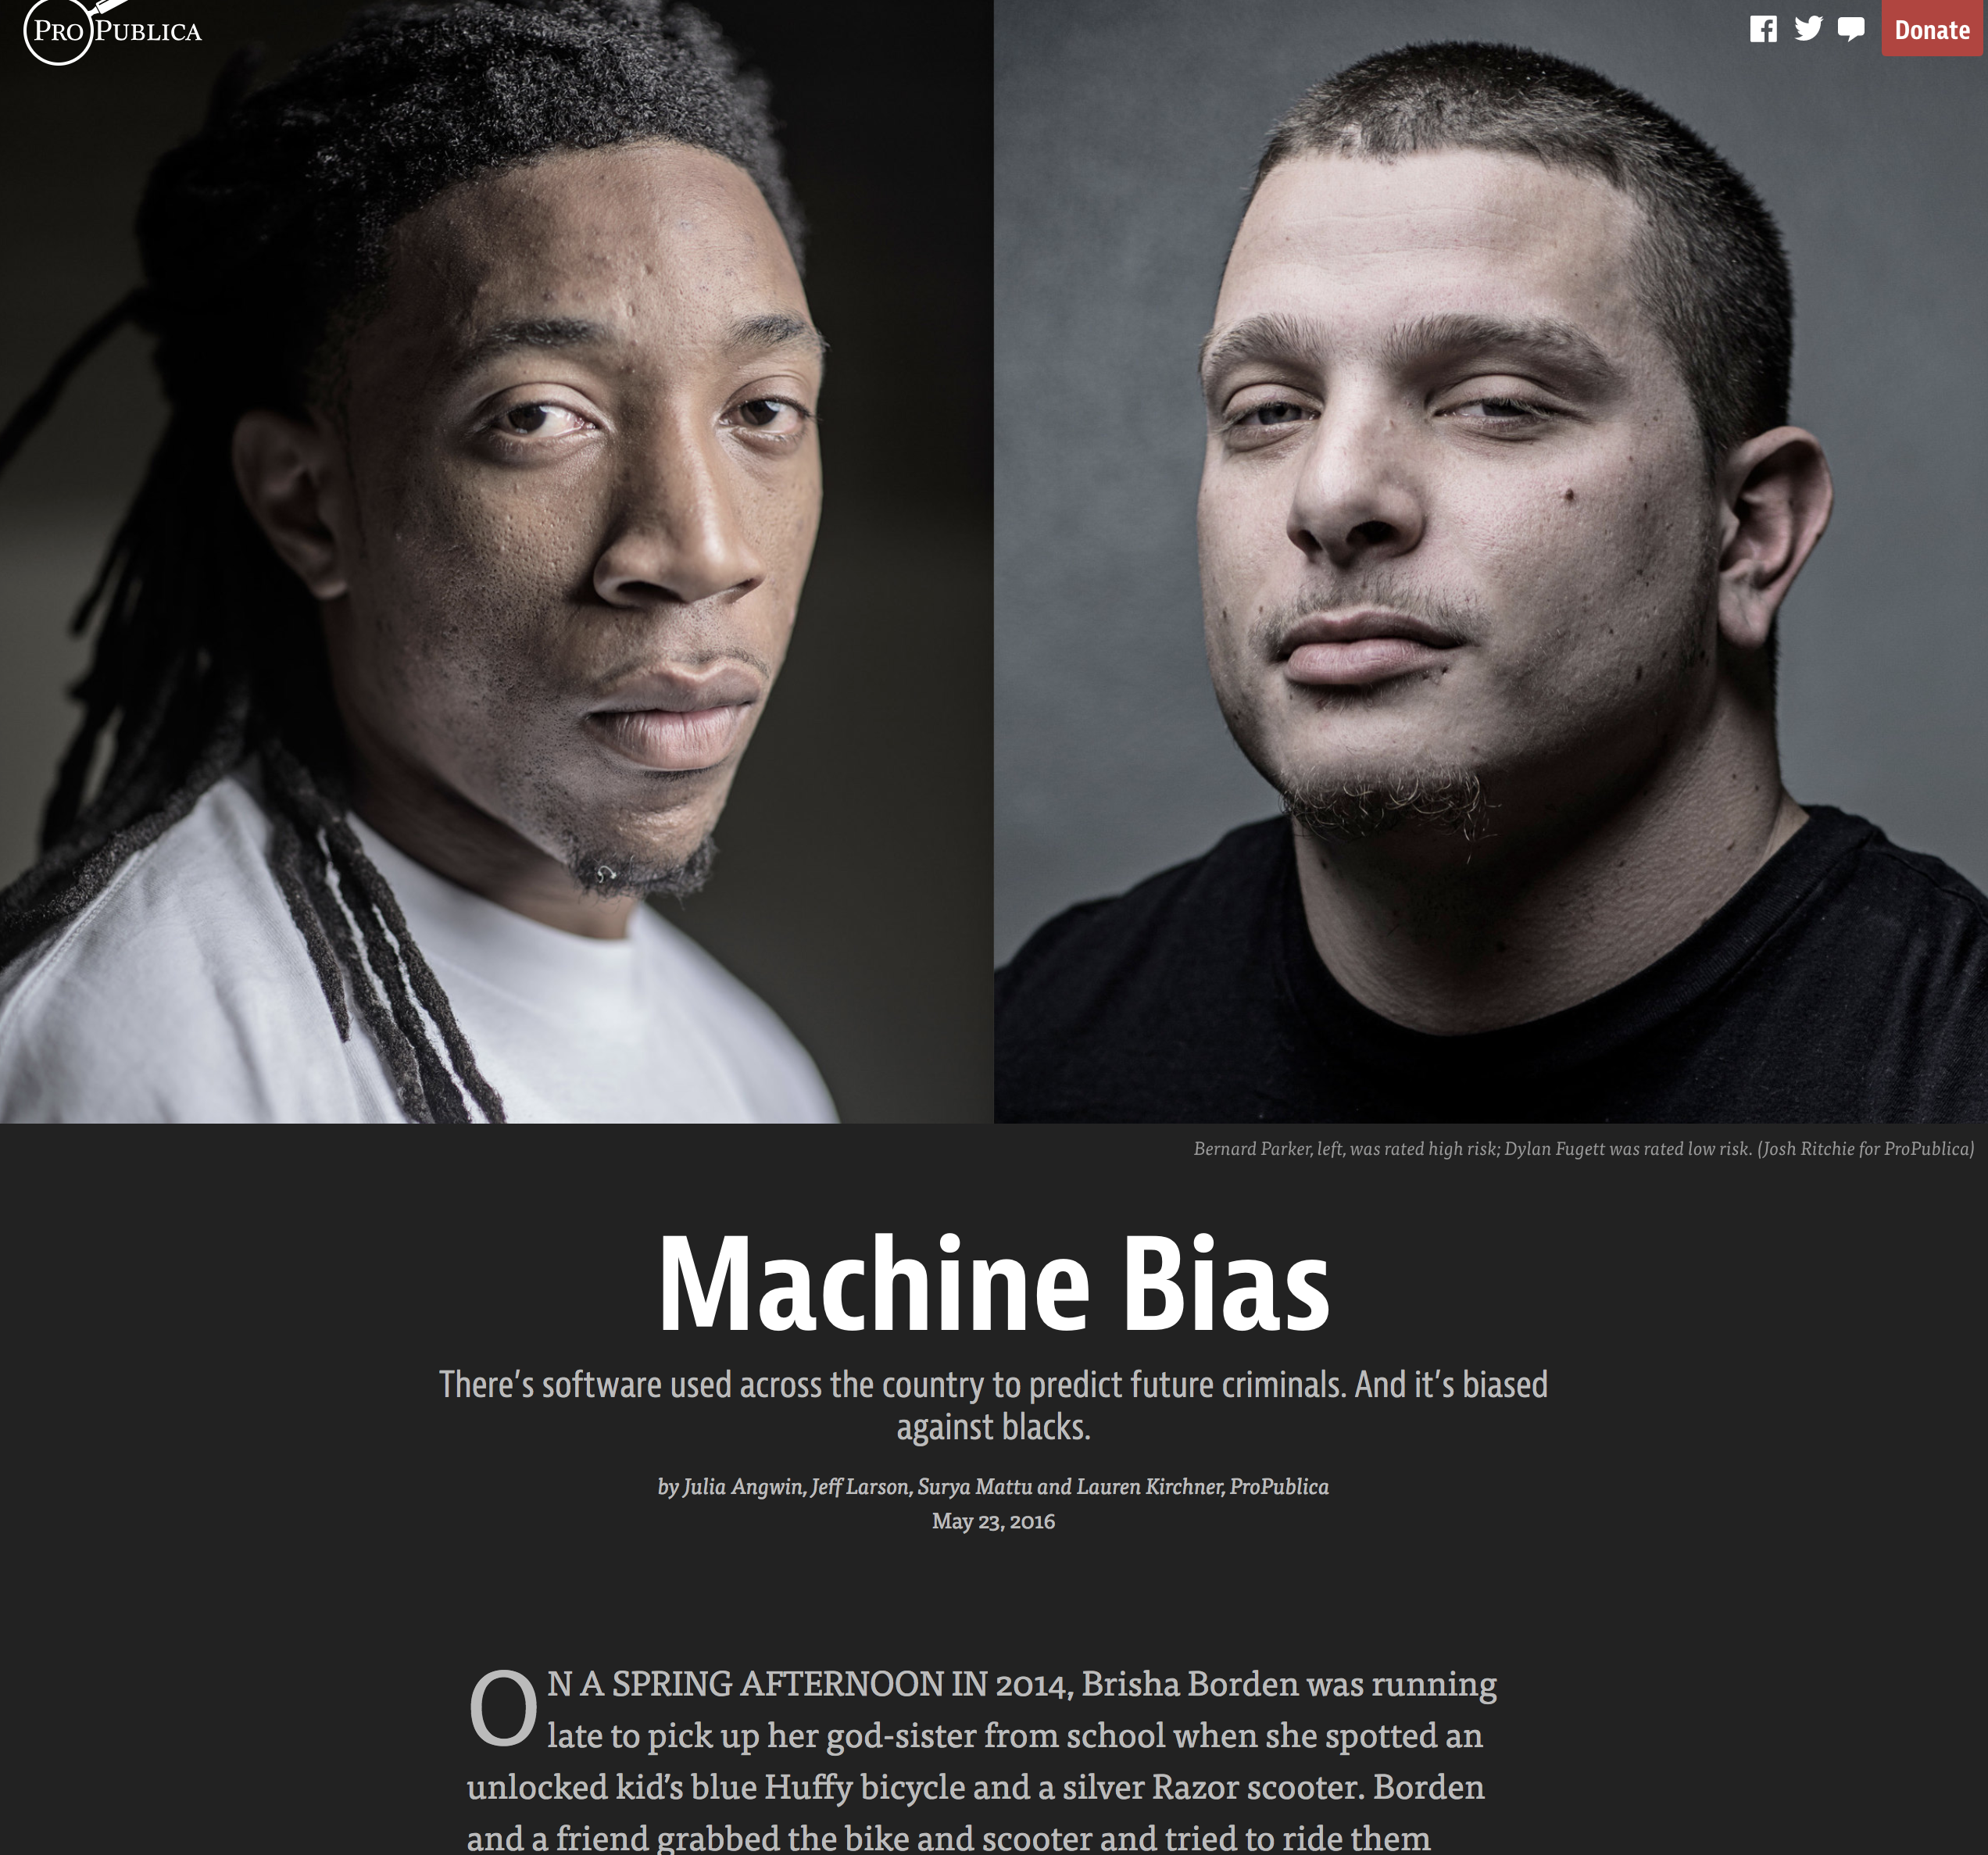
\includegraphics[max width=\linewidth,keepaspectratio]{figures/court_bias.png}
%     \end{column}
%     \begin{column}{0.49\textwidth}
%       \centering
%       \includegraphics[max width=\linewidth,keepaspectratio]{figures/court_more.png}
%     \end{column}
%   \end{columns}
% \end{frame}


% \begin{frame}{Creativity in crowdwork}
%   \begin{columns}[T]
%     \begin{column}{0.33\textwidth}
%       \centering
%       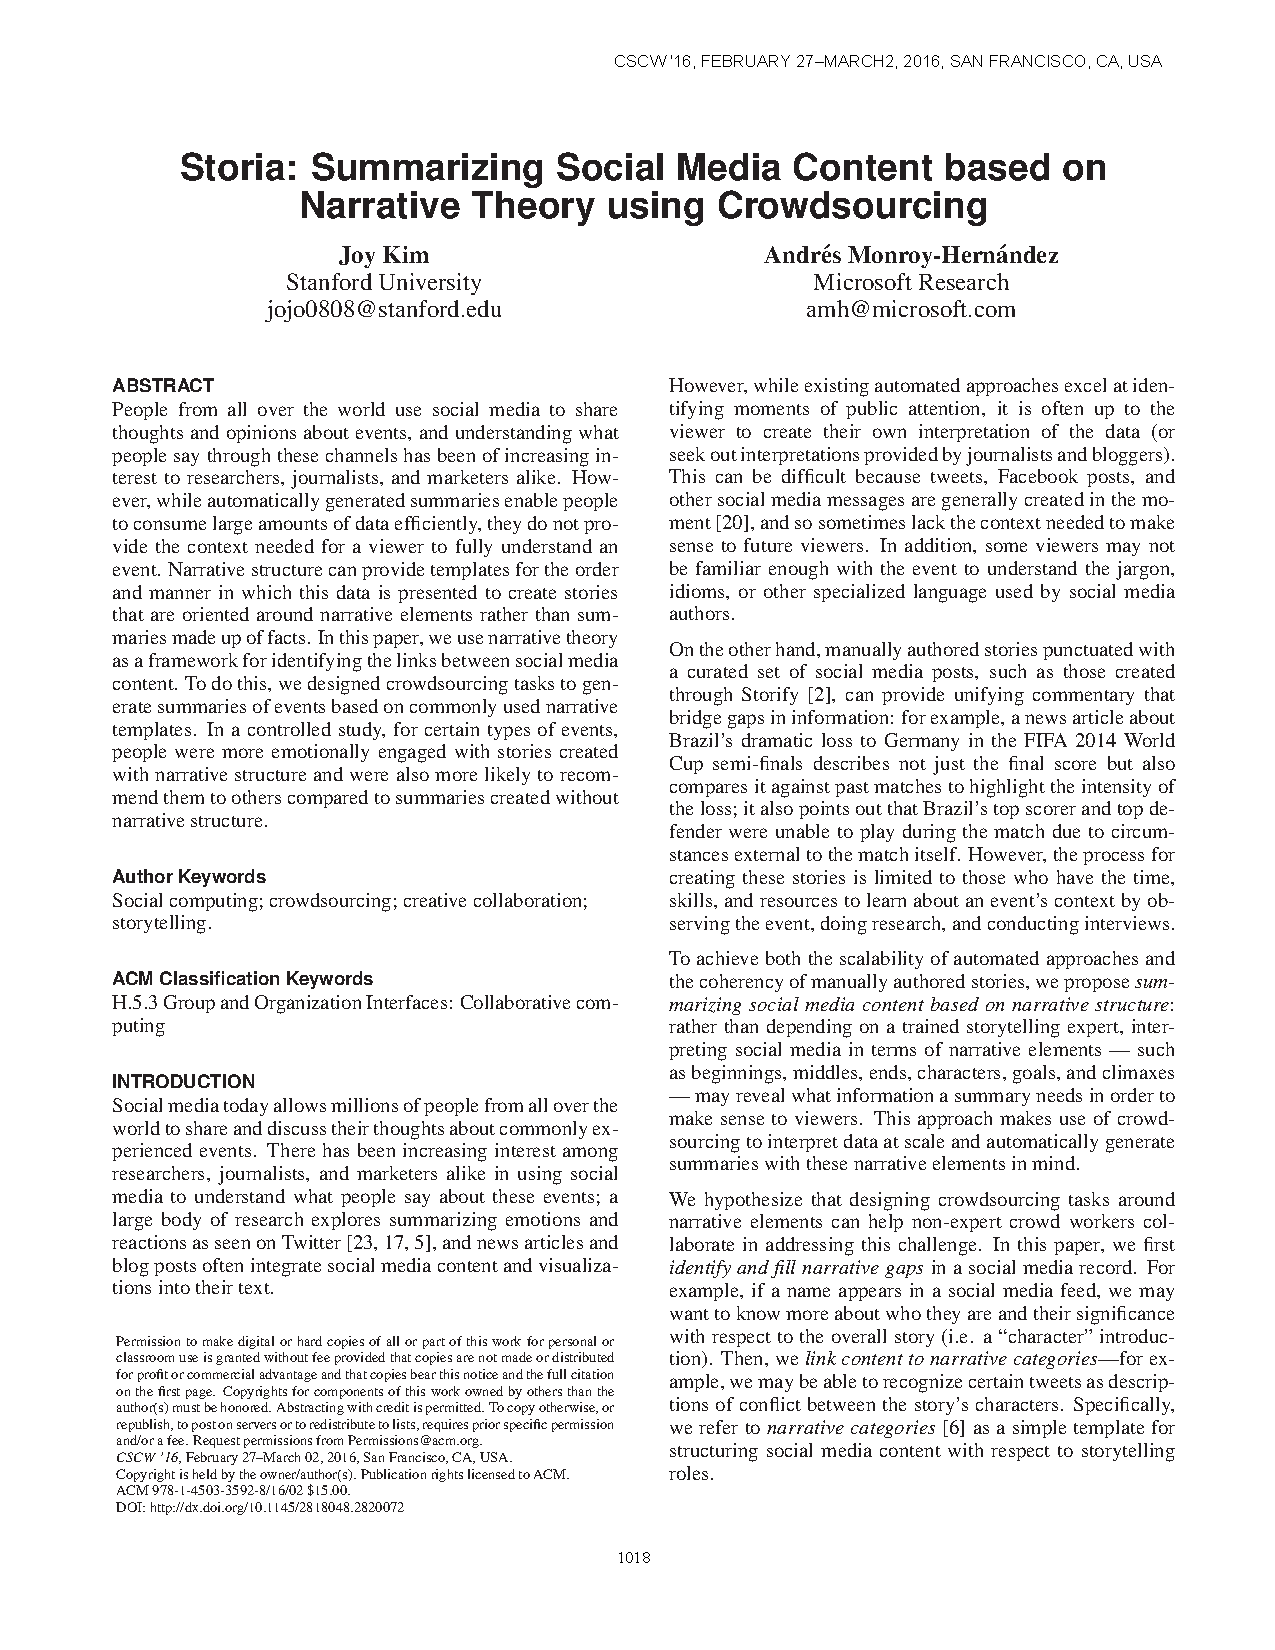
\includegraphics[max width=\linewidth,keepaspectratio]{figures/1018_kim.pdf}
%     \end{column}
%     \begin{column}{0.33\textwidth}
%       \centering
%       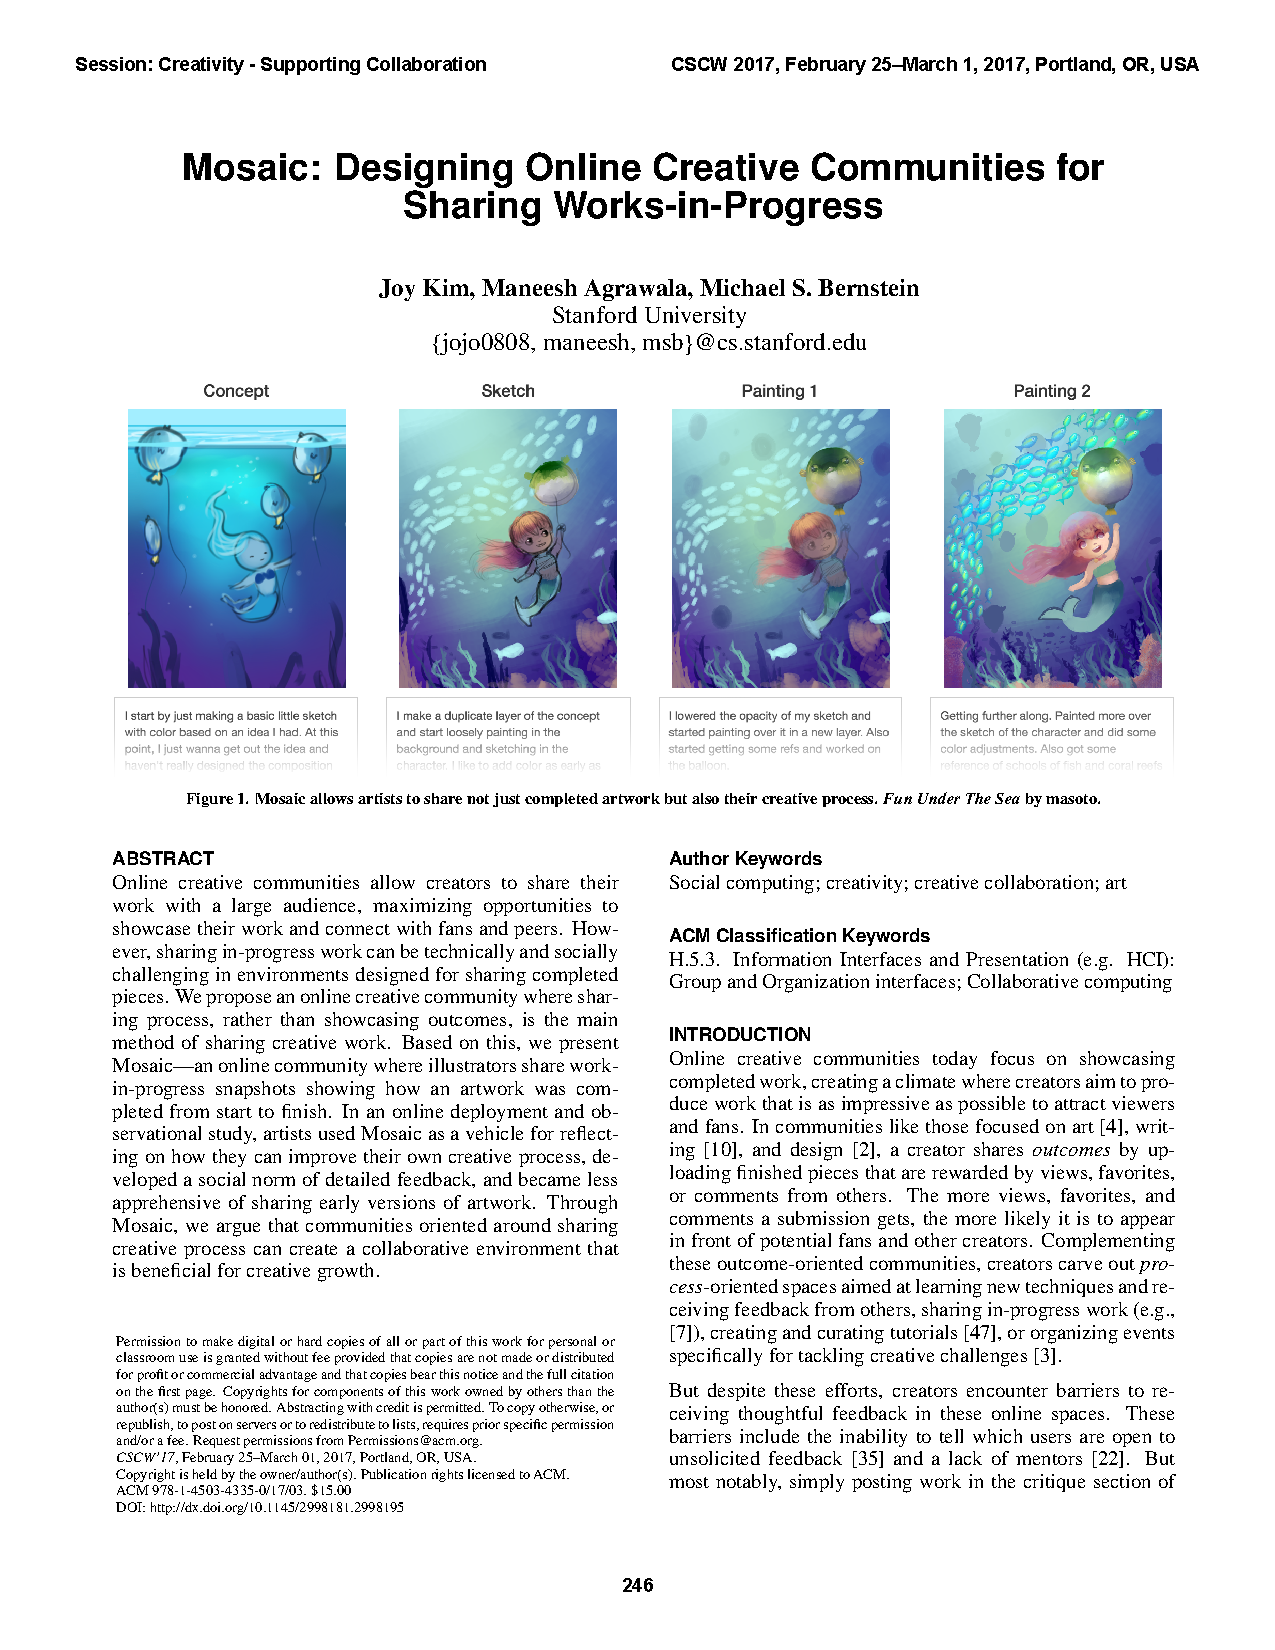
\includegraphics[max width=\linewidth,keepaspectratio]{figures/p246-kim.pdf}
%     \end{column}
%     \begin{column}{0.33\textwidth}
%       \centering
%       \includegraphics[max width=\linewidth,keepaspectratio]{figures/p233-kim.pdf}
%     \end{column}
%   \end{columns}
% \end{frame}


% \begin{frame}<1>[t,label=pieceworkreveal]{Outlining the landscape}
%   \visible<3->{
%   \begin{columns}[T]
%     \begin{column}{0.33\textwidth}
%       \centering
%       \includegraphics[max width=\linewidth,max height=.3\textheight,keepaspectratio]{../common_figures/pieceworkers.jpg}
%     \end{column}
%     \begin{column}{0.33\textwidth}
%       \centering
%       \includegraphics[max width=\linewidth,max height=.3\textheight,keepaspectratio]{../common_figures/photo/ford_assembly_line.jpg}
%     \end{column}
%     \begin{column}{0.33\textwidth}
%       \centering
%       \includegraphics[max width=\linewidth,max height=.3\textheight,keepaspectratio]{../common_figures/photo/Rosie_the_Riveter_(Vultee)_DS.jpg}
%     \end{column}
%     % }
%   \end{columns}
%   \vspace*{7mm}
%   }
  
%     \begin{columns}[b]
%       \begin{column}[t]{0.45\textwidth}
%         \centering
%         Crowd work
%         \begin{columns}
%           \begin{column}[b]{.5\textwidth}
%             \includegraphics[max width=\linewidth,max height=\textheight,keepaspectratio]{../common_figures/amt.png}
%           \end{column}
%           \begin{column}[b]{.5\textwidth}
%             \includegraphics[max width=\linewidth,max height=\textheight,keepaspectratio]{../common_figures/upwork.png}
%           \end{column}
%         \end{columns}
%       \end{column}

%       \begin{column}[t]{0.45\textwidth}
%         \centering
%         Gig Work
%         \begin{columns}
%           \begin{column}{.5\textwidth}
%             \includegraphics[max width=\linewidth,max height=\textheight,keepaspectratio]{../common_figures/uber.png}
%           \end{column}
%           \begin{column}{.5\textwidth}
%             \includegraphics[max width=\linewidth,max height=\textheight,keepaspectratio]{../common_figures/postmates.png}
%           \end{column}
%         \end{columns}
%       \end{column}
%     \end{columns}
% \end{frame}

% \begin{frame}[standout,label=takeaway]{Provocation \#0}
%   On--demand work is a modern instantiation of a much older phenomenon

% \vspace{2em}
%   \visible<2->{\alert{piecework}}

% \end{frame}

% \againframe<2->{pieceworkreveal}

% \begin{frame}[standout]{provocation \#1}
%     What is work going to look like in the future?
% \end{frame}
\end{document}